\section{Resultados}

Nesta seção, deverão ser apresentados os resultados do trabalho realizado. Vocês podem inserir imagens no trabalho, conforme o código abaixo:

\begin{figure}[htp]
    \centering
    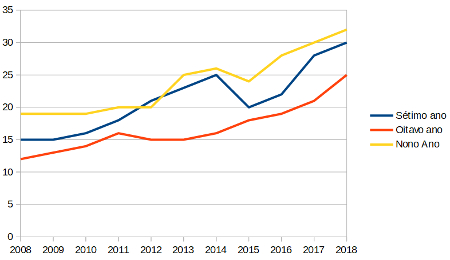
\includegraphics[width=10cm]{imagens/grafico.jpg}
    \caption{Um gráfico como exemplo.}
    \label{fig:galaxy}
\end{figure}

Vocês também podem trabalhar com equações matemáticas com bastante destreza no Latex.

\[ x^n + y^n = z^n \]

Podemos trabalhar, obviamente, com expressões um pouco mais cabulosas:

$$\lim_{x\to\infty} f(x)$$

$$\sum_{n=1}^{\infty} 2^{-n} = 1$$	

$$\oint_V f(s) \,ds$$

Apesar de um pouco complexo, é possível trabalhar com tabelas no Latex, como pode-se ver com o código a seguir:

\begin{tabular}{ |p{3cm}||p{3cm}|p{3cm}|p{3cm}|  }
 \hline
 \multicolumn{4}{|c|}{Lista de Países} \\
 \hline
 Nome do País ou Área& Código ISO Alpha 2 & Código Alpha 3& Código Numérico Alpha\\
 \hline
 Afghanistan   & AF    &AFG&   004\\
 Aland Islands&   AX  & ALA   &248\\
 Albania &AL & ALB&  008\\
 Algeria    &DZ & DZA&  012\\
 American Samoa&   AS  & ASM&016\\
 Andorra& AD  & AND   &020\\
 Angola& AO  & AGO&024\\
 \hline
\end{tabular}

Para conhecer um pouco mais sobre as funcionalidades do ambiente, não deixe de acessar a documentação em \url{https://www.overleaf.com/learn/latex/Main_Page}.
